\documentclass{article}

\usepackage{amsthm,amsmath,amssymb}
\usepackage[numbers]{natbib}
\usepackage{hyperref}
\usepackage{graphicx}
\usepackage{caption}
\usepackage{subcaption}
\newcommand{\bx}{{\mathbf x}}
\newcommand{\by}{{\mathbf y}}
\newcommand{\ba}{{\mathbf a}}
\newcommand{\bv}{{\mathbf v}}
\newcommand{\bu}{{\mathbf u}}
\newcommand{\bw}{{\mathbf w}}


\newtheorem{theorem}{Theorem}[section]
\newtheorem{proposition}[theorem]{Proposition}
\newtheorem{lemma}[theorem]{Lemma}
\newtheorem{corollary}[theorem]{Corollary}
\newtheorem{remark}{Remark}[section]
\newtheorem{example}[theorem]{Example}


\begin{document}

\title{Management Sciences Topics: Convex Optimization\\ Homework 4: Due April 18rd (11:59 pm) }
%\author{Qihang Lin}
\date{}

\maketitle
\noindent(You can directly use any properties, theorems, examples or facts from the lectures.)
\bigskip

\noindent\textbf{Problem 1:}  Apply the Extra Gradient method to solve the (overlapping group regularized logistic regression) problem in Problem 2 of Homework 3. You need to use the same dataset and the same setup of the problem. Plot the primal objective values in each iteration.
\bigskip

The code for this problem is \texttt{extra\_gradient.m} and \texttt{problem1.m}. The result is shown as follows.

\begin{figure}[h]
\centering
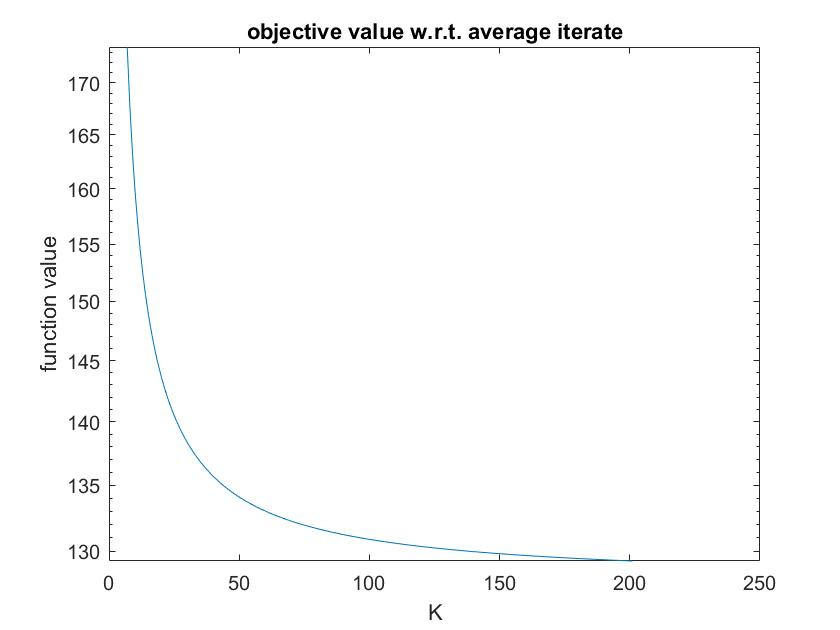
\includegraphics[scale=0.3]{problem1.jpg}
\label{problem1-result}
\caption{Primal objective value for problem 1.}
\end{figure}

\noindent\textbf{Problem 2:} Apply both the Extra Gradient method and the Primal-Dual Subgradient method to the following two-person-zero-sum problem. 
\begin{eqnarray*}
\min_{\bx\in\mathcal{X}}\max_{\by\in\mathcal{Y}}\by\top A \bx
\end{eqnarray*}
where $A$ is an $m\times n$ matrix, $\mathcal{X}\subset\mathbb{R}^n$ and $\mathcal{Y}\subset\mathbb{R}^m$ are simplexes in their own space. You need to download the matrix $A$ from ICON. It is in the file named ``two-person-zero-sum.mat''.
\bigskip

The code for this problem is \texttt{projection\_on\_simplex.m}, \texttt{problem2.m}. The result is shown as follows, where the left plot is the result of extra gradient method and the right is of primal-dual subgradient method.

\begin{figure}[h]
\centering
\vbox{
	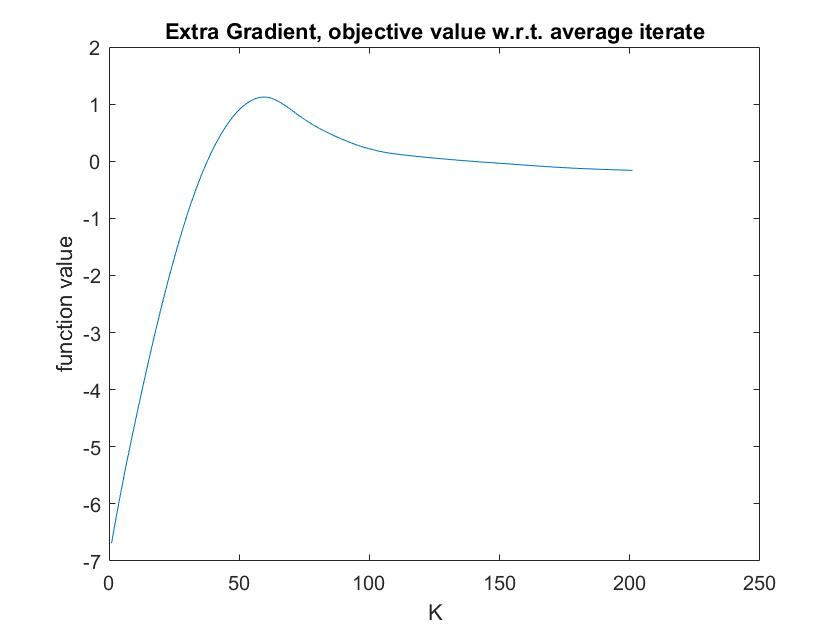
\includegraphics[scale=0.2]{problem2_extra_gradient.jpg}
	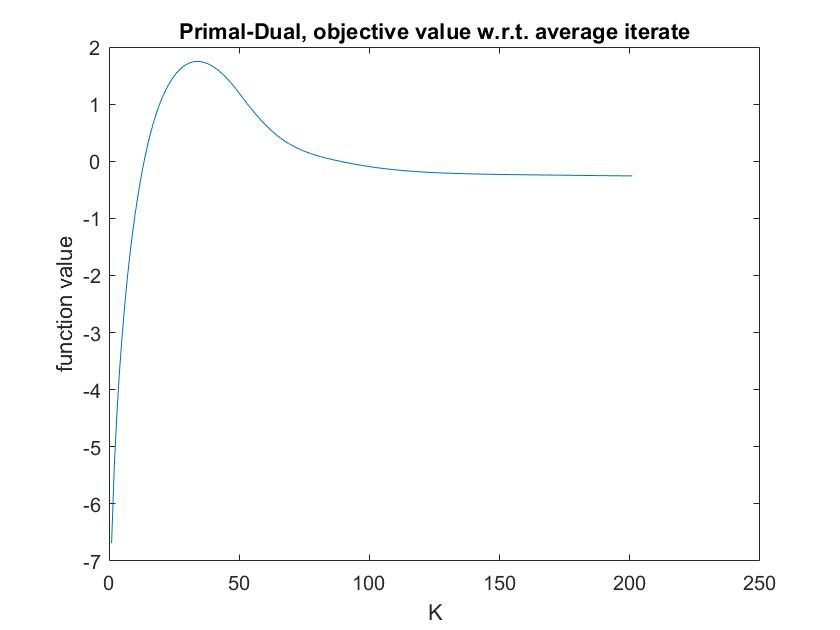
\includegraphics[scale=0.2]{problem2_primal_dual.jpg}
}
\label{problem2-result}
\caption{Primal objective value for problem 2, where the left plot is the result of extra gradient method and the right is of primal-dual subgradient method.}
\end{figure}


\noindent\textbf{Problem 3:} Apply the level-set method to solve the following Danzig Selector problem
\begin{eqnarray*}
\min_{\bx_+,\bx_-}&& \mathbf{1}^\top(\bx_++\bx_-)\\
\text{s.t.} &&0\leq \bx_+,\bx_-\leq 10\\
&& -10\leq A^\top(A(\bx_+-\bx_-)-b)\leq 10,
\end{eqnarray*}
where $A$ and $b$ are the feature matrix and the output vector of the dataset ``triazines'' from LIBSVM library. You must use the scaled version (``triazines\_scale'').
\url{https://www.csie.ntu.edu.tw/~cjlin/libsvmtools/datasets/regression.html#triazines}
Use the Extra Gradient method 
\bigskip
\end{document}

